\chapter{Sequential fitting}\label{Chap:Sequential}

Back in the old days, a Rietveld fit was a one-to-one thing. You had sample that was composed of a single phase, you collected a set of powder diffraction data and one fit the structure (and all the other parameters this book discusses) to the data. So, one dataset and one phase: one refinement. The first change in that was that the software was expanded to handle fitting a second phase, so binary mixtures could then be fit. In the 1980s, the original GSAS came along, which could handle what then seemed to be an infinite number of phases -- nine.\footnote{The reason for the limit of 9 was partly because Fortran required fixed memory allocations, so if you created an array with 500x20x4 elements (say for 500 atoms and 20 phases and 4 coordinates/Uiso values) that would lock up 156 Kbytes and back then you cared about what is now considered a tiny bit of memory; but, the other reason was that in the files only a space for a single digit was allowed in the place where the phase number was written.} GSAS also allowed you to read in 99 histograms (two digits!) and GSAS could fit your 9 phases simultaneously to all the datasets as you had loaded. This allowed something quite new. One could simultaneously fit a single crystal structure to more than one type of data. I can recall a structure containing both vanadium and deuterium, where V is pretty much invisible to neutrons, and x-rays have real difficulty with H (or D) atom positions. We had single-crystal x-ray data and I collected a neutron powder diffraction patterns, and did a combined fit to the two datasets. It worked great and an excellent fit was obtained to both sets of measurements. This was much better than what would have been done before GSAS came along, which would have been to fix some of the structural information in the Rietveld fit to results from the single-crystal fit. The quality of the combined fit was much better. Another example from my own work of the revolution wrought by GSAS is discussed in Section \ref{ref:CaLSX}, where I used a synchrotron x-ray and neutron dataset together for a ``simple'' zeolite sample. 

Since the 1990's there has been a second revolution, and that is in the speed that one can collect powder diffraction data. A typical neutron powder diffraction pattern required at least a 12 hour measurement, likewise about the same for a high-resolution synchrotron powder diffraction pattern. Use of a PSD brought that down to 3-4 hours. Now, under the best circumstances, one can collect a neutron diffraction pattern in fraction of an hour and a medium-resolution synchrotron dataset in a fraction of a second; a high-resolution pattern in minutes. This allows for parametric measurements, where large numbers of diffraction patterns are collected while changes are made to the sample: different samples can be used or the temperature, pressure, chemical environment, electrostatic potential,... are varied. For non-equilibrium conditions, cycling the conditions may show systematic changes. A single experiment can result in thousands of powder diffraction patterns. To plan for this data deluge, with GSAS-II we designed a mechanism called sequential fitting for refinements for fitting similar models to large numbers of datasets. The original approach, where one model is fit simultaneously to all datasets, I will call a combined refinement, even if the model is a single phase and the data are a single histogram.

\section{What is a sequential fit?}
In a sequential fit is one where a fit is performed independently for a set of phases using one dataset after another. This is in contrast to a combined fit, where all phases are fit to all datasets. In a combined fit, if more than one histogram is present and each is linked to one or more phases, all linked phases will be fit to all linked and ``Used''\footnote{Where the ``Use flag'' is turned on.} histograms.  Phases that are not linked to histograms are ignored. Likewise, histograms where the ``Use flag'' is turned off or that are not linked to any phases will also be ignored. 
The difference between the two is in how the models are parameterized. In a combined fit, there are separate histogram parameters for each histogram and separate HAP parameters (HAP parameters are  explained in section \ref{ref:HAP}) for each phase and histogram, but only one set of phase parameters must fit all histograms. Thus, when several histograms are fit, 
the atom positions and ADP values will represent a compromise that best-fits all histograms simultaneously. This it is some sort of average. This is often optimal. In a sequential fit, each dataset will have individually-fit parameters, so atoms positions and ADP values can evolve as the datasets change parametrically, for example, as the temperature is changed. 
Note that, as will be discussed later in section \ref{ref:dij-seq}, lattice parameters can be fit separately in either refinement type so lattice parameters are not forced to be the same for every dataset in either type of fit. 
In both cases, it is possible to designate which phases are associated with individual histograms, so it is possible to model cases where phases appear or disappear. 
Sequential refinements offer one additional result: a table is prepared with the fit parameters showing how they change, as will be discussed in Section \ref{ref:seqres}. There are  a number of nice tools to follow the progress of the fits. 
A good resource for learning about sequential refinements can be found in the ``Sequential refinement of multiple datasets – CuCr2O4 from 7K to 300K'' tutorial, 
\url{https://advancedphotonsource.github.io/GSAS-II-tutorials/SeqRefine/SequentialTutorial.htm}. A second tutorial, ``Parametric Fitting and Pseudo Variables for Sequential Fits'', 
\url{https://advancedphotonsource.github.io/GSAS-II-tutorials/SeqParametric/ParametricFitting.htm}, 
shows some of the tools that GSAS-II provides from the results of a sequential fit. 
The goal of this chapter is not to duplicate those tutorials, but to explain how sequential fitting works and discuss different ways that sequential fitting can be approached.

There are a few important concepts that are worthwhile to discuss before considering the mechanics of performing a sequential fit. 


\subsection{Switching to a sequential fit}
By default in GSAS-II, a combined fit is performed. To establish that a sequential fit will be performed, you need to select the Controls data tree entry and in the middle of the data window, as seen in Fig. \ref{fig:seq0} click on the Sequential Settings ``Select datasets'' button. This brings up a window where you can select histograms. If you select one or more histograms, sequential mode is enabled. Why one might want to perform a sequential fit with only a single histogram will be made more clear later, in  Section \ref{ref:prepseq}.
\begin{figure}
    \centering
    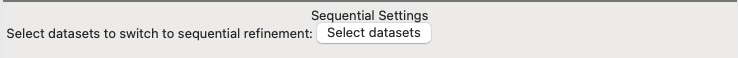
\includegraphics[width=0.75\linewidth]{figures/seq0.jpg}
    \caption{Switching to sequential mode: the ``Select datasets'' button shown here (accessed on the Controls data tree entry) is used to select histograms to be included in a sequential fit. This turns on sequential mode.}
    \label{fig:seq0}
\end{figure}
Once sequential mode is entered, this section of the data window changes, as seen in Fig. \ref{fig:seq1}.  Also, the ``Refine''command in the Calculate menu is replaced with ``Sequential refine.'' 
\begin{figure}
    \centering
    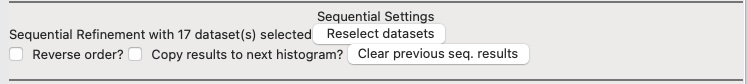
\includegraphics[width=0.75\linewidth]{figures/seq1.jpg}
    \caption{Once Sequential mode is entered, the Controls data tree entry appears as shown here. }
    \label{fig:seq1}
\end{figure}
The new controls that are available are: 
\begin{itemize}
    \item ``Reselect datasets'' button: You can change which datasets are included in the sequential fit with this. If for some reason you would want to turn off sequential mode, use this, but do not select any datasets before pressing OK. 
    \item ``Reverse order?'': When this is unselected, the selected datasets are processed in the order they appear in the data tree (top down). When this is selected the order is reversed (bottom to top).
    \item ``Copy results to next histogram?'': When this is selected, the fitted parameters at the end of one fit are used as the starting point for the next histogram. After a sequential fit is performed, this is always turned off. The use of this is discussed in more depth in Section \ref{ref:copynext}.
    \item ``Clear previous seq. results'' button: Results from a sequential fit are placed into a data tree entry. This button deletes that data tree entry from the GSAS-II project. This is discussed in more depth in Section \ref{ref:seqres}.
\end{itemize}

Note that when a sequential fit is established, only the histograms included in the list of selected  dataset are used in a refinement. All others are ignored. Thus, a sequential fit can be performed in stages, where datasets are added in stages. 
This is  different from the combined fit process, where all histograms that are linked to one or more phases will be used in the fit unless their ``Use'' flag is set to off. 

\subsection{Lattice parameter offsets}\label{ref:dij-seq}
A key change between combined and sequential fit has to do with how lattice parameters are treated in GSAS-II.
Note that a phase has only a single set of lattice constants, so these constants alone will not treat the case where a phase description is being used to fit multiple datasets where the data were collected under different conditions as the lattice parameters are likely to not be identical at the great sensitivity that Rietveld refinement offers. 

As was introduced in Section \ref{ref:Dij}, a hydrostatic strain tensor, $D_{ij}$, allows for delta values to be applied to lattice constants. These $D_{ij}$ values are HAP values, so there is a set of them for every histogram associated with a phase. The effect of these terms is that lattice parameters are being treated as $a = a_0 + \delta a_j$ where $a_0$ is the lattice parameter associated with the phase, and there is an offset $\delta a_j$ associated with each histogram, except the $D_{ij}$ terms are actually applied to the reciprocal lattice tensor. I will leave deriving an expression for $\delta a_j$ from the $D_{ij}$ terms in the general triclinic case ``as an exercise for the reader.'' (No partial credit for the cubic case.) An example showing how the lattice parameters and the $D_{ij}$ terms are displayed in the GUI is shown in Figs. \ref{fig:dij1} and \ref{fig:dij2}, respectively.
\begin{figure}
    \centering
    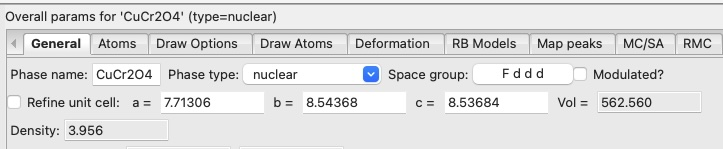
\includegraphics[width=0.8\linewidth]{figures/Dij1.jpg}
    \caption{Lattice parameters for an example phase. Note that these values may be refined in a combined fit, but are not refined in a sequential fit.}
    \label{fig:dij1}
\end{figure}
\begin{figure}
    \centering
    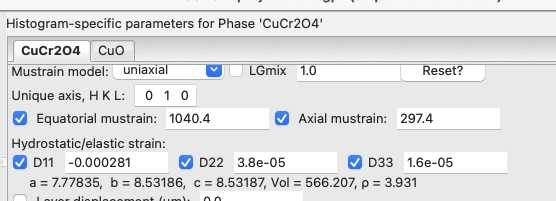
\includegraphics[width=0.6\linewidth]{figures/Dij2.jpg}
    \caption{Hydrostatic strain tensor ($D_{ij}$) values from a sequential fit. These values are sometimes refined for some phases in a combined fit and are almost always refined in a sequential fit. Note that this shows how the $D_{ij}$ change the lattice parameters from what is shown for the phase in Fig. \ref{fig:dij1}. Note that these parameters are found in the Data tab for the phase, unless the HAP items are placed directly into the Hist/Phase data tree entry (see section \ref{ref:separatehistogram}).}
    \label{fig:dij2}. 
\end{figure}
These hydrostatic strain tensor ($D_{ij}$) terms are essential for sequential fits. Should you attempt to refine the lattice parameters in a sequential fit, a warning message will be displayed and the software will offer to turn off the lattice parameter flag and turn on refinement of the $D_{ij}$ terms. The software will not allow a sequential refinement where lattice parameters are refined directly.

\subsection{Use of ``Copy results to next histogram?''}\label{ref:copynext}.
When performing a parametric refinement, a model that fits the first dataset may not be a good starting point for a data set collected much later in the series. For example, the lattice parameters may have changed sufficiently, that the peak positions no longer are close enough to the computed reflection positions that refinement can progress.\footnote{Remember that unless there is at least some overlap between observed and computed for at least one peak with a non-zero value for \textit{h}, \textit{k} and \textit{l}, the likelihood is high that the refinement will fail to find the correct lattice parameters. If the lattice parameters are wrong, the fit is wrong.} This ``Copy results to next histogram'' option will take the results from the fit of histogram $n$ and copy those parameters as the starting point for histogram $n+1$. Even if the starting point parameters in a parametric fit would be close enough for a fit to progress, if the datasets are showing a orderly progression in changes, starting from an adjacent set of parameters will cause a more rapid convergence. 

Note, however, that you will only want to use this option for the first time that a set of histograms are fit. Once the a refinement has been run on a set of histograms, the initial values have been optimized and use of this option would reset the parameters, which is probably not what you want. For this reason, the ``Copy results to next histogram?'' setting is automatically cleared after a sequential fit is performed. However, if you are performing a sequential fit in stages, you may want to turn this back on when you select a new set of histograms to use in a sequential fit.


\section{Preparing for a sequential fit}
Some sequential fits will be for a series of datasets where the same refinement settings will be optimal for all of the histograms. The tutorial is an example of that. However, this is not always the case. As one example, if during a set of diffraction measurements, a new phase appears, you will need to change the refinement settings to include that phase at the point in the sequence where that phase is first seen. When the phase first appears, there may be too few peaks to refine more than the phase fraction. Once more peaks are present, you will likely wish to refine the lattice parameters. At a later stage, you may want to refine structural and/or sample broadening terms. 

Unless your datasets are all very similar, you will likely want to add parameters to the model as the refinement progresses. Note that after you set the refinement flags in the data window for any histogram or HAP data tree item, there is a menu item for ``Copy flags.'' This will allow you to set the same refinement flags for other histograms without having to visit the data tree item for each histogram. The hard part is remembering to use the ``Copy flags'' menu command, but if you fail to do this, you can simply copy them in the next refinement. Note that in most of the menus, there is also a ``Copy'' and a ``Copy Selected'' menu command. The ``Copy'' or  ``Copy parameters'' will copy all parameters and their refinement flags (with the exception that for Sample Parameters, only the refined values and a few other items, such as instrument name are copied; values that are expected to change such as temperature, setting angles, etc. are not copied.) You will be asked to which histograms to copy the values. The ``Copy Selected'' menu command offers a choice of which parameters to copy as well as the histograms to where they will be copied. For both cases the values that will be copied are coming from the currently-selected histogram. 

There are two schools of thought about how to perform sequential fits. One is to review the data and look for where there are significant changes and to use that knowledge to group the histograms into sections that are likely to work well with the same refinement settings. The other is to find reasonable settings for the fit of the first histogram and then let the sequential fit go and see where it starts to fail  as an indication of where the refinement settings need to change. Both approaches work. Personally, I prefer to know more about what is going on in my data. 

\section{Starting a sequential fit}\label{ref:prepseq}
Before starting any fit, one must import phases, link them to histograms, ensure that lattice parameters are sufficiently close that refinement will progress, set up a background model, etc. The steps needed here have been discussed in the chapters in \ref{sect:PatternFitting}. At a minimum, you will want to place some special attention onto the refinement of the first dataset in a sequential fit. As noted, you may want to do this with several different histograms across the series of measurements. How this will be done is also a personal style. In the tutorial, a GSAS-II project is created with a single histogram and two phases. This refinement is performed as a standard combined fit and after that is done, additional histograms are added and the refinement is set to be a sequential fit. It is also possible to start that fit by importing the entire sequence of datasets and then to initially select a sequential fit for just the first dataset until you are ready to progress to a fit of all datasets. 

\section{Sequential fit results table}\label{ref:seqres}
When a sequential fit is performed, the results from that fit are placed into a new data tree entry, the Sequential Results, where the associated data window shows a table with the results from the fit. Each histogram has a separate row. An example of this is shown in Fig. \ref{fig:seqrestbl}. The first few columns in the table show values that track the refinement progress and sample parameters that change between histograms. The $\Delta\chi^2$ value is of particular value to know if the refinement has converged. This shows the change in the overall $\chi^2$ value before and after the last refinement as percentage. If this number is more than a percent or so, the refinement is still showing significant changes. If very large, you may want to repeat the refinement before varying additional parameters. For the final run, you want al; these values to be well under a percent. Larger values are highlighted in color to make them more obvious. 

Later columns of the table show lattice parameters, when these are refined, and then later columns show refined parameters. Note that the ``Hide columns...'' command in the ``Columns/Rows'' menu is used to select the refined parameters that are included. 
\begin{figure}
    \centering
    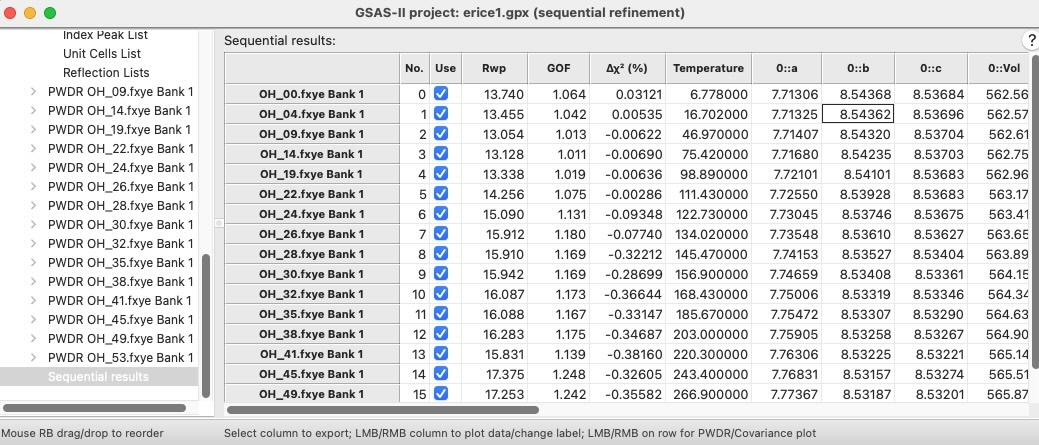
\includegraphics[width=0.9\linewidth]{figures/seqrestbl.jpg}
    \caption{A sample sequential results table.}
    \label{fig:seqrestbl}
\end{figure}
There are a lot of tools programmed for use with this table. Note that allowing the mouse to ``rest'' (allow the mouse to stay in one position for a few seconds) on a column heading will display some information about that column; allowing it to rest on a value in the table, will show that s.u. value, if one exists. Clicking on a column plots the values in that column. Selecting more than one column will plot those values together. The default x-axis values are the sequence numbers for each histogram, but pressing the ``s'' key in the plot (or using the ``K'' button on the plot toolbar and then selecting the ``s'' option) causes a list of columns to be shown. By selecting, for example, the temperature column, values can be plotted against temperature. Clicking on a row heading causes the histogram fit to be displayed and right-clicking on the heading shows the correlation matrix plot. 

The ``Pseudo Vars'' menu commands allow you to compute values from the fitted parameters, which can be a distance between atoms or a formula that you specify, such as the ratio of lattice parameters. An example of this is in the 
``Parametric Fitting and Pseudo Variables for Sequential Fits'' (\url{https://advancedphotonsource.github.io/GSAS-II-tutorials/SeqParametric/ParametricFitting.htm}) tutorial. These computed values are added to the table and are recomputed each time the table is shown. The s.u. for these values is computed. These values can also be used as the x-values for plotting. So, for example, should you wish to plot against temperatures in Celsius rather than Kelvin, you can create a pseudo-var that subtracts 273.15 from the temperature and then use that for plotting. 

You can also use the ``Parametric Fit'' menu commands to define an equation that will be fitted to the values in the sequential table. This is also demonstrated in the ``Parametric Fitting and Pseudo Variables for Sequential Fits'' (\url{https://advancedphotonsource.github.io/GSAS-II-tutorials/SeqParametric/ParametricFitting.htm}) tutorial. Uncertainties in parameter values, as well as the parameters' covariance are taken into account during fitting. 

Note that if histograms are removed from the sequential dataset list, their results are not removed from the table. Thus, this table can be built up in sections. However, if one want to omit values from a histogram from being used in calculations and plots, unselect the ``Use'' flag in the second column. That will effectively remove that row from consideration. 
It is recommended that after all histograms have been successfully refined, a final fit be performed that includes all histograms, but this should not actually change the results in any meaningful way. 

\section{Parametric fitting}
As was shown in Section \ref{ref:seqres}, we can fit an equation of state to the results of a parametric fit. You might think it better to build the equation of state into the model and then fit that equation of state directly to all the data.
As an example of this, one could define an equation that fits the volume expansion as a function of temperature to straight line and then rather than fitting the individual lattice constants, the thermal expansion coefficients would be fit directly, as has been done with other software. Since all the lattice constants are reduced to two linear thermal expansion coefficients, such a fit will appear to have much less ``jitter'' in the individual fits. Nonetheless, I feel that building a parametric equation into the fit is a poor choice. First of all, the two-step process we use, where least-squares fitting is done to the results from least-squares has been demonstrated (by Ted Prince\index{Prince, E.}) to produce the exact same results as a single fit, provided that the full covariance matrix is taken from the first fit and used in place of weights in the second fit. Since each fit in a sequential fit is independent, the only covariance that needs to be considered is that for the parameters that are fit together, and this is done in parametric fitting. However, the more important reason is that when a parametric equation is ``baked into'' a model, it becomes a constraint. It becomes very difficult to see that the constraint is not correct. If one constrains linear expansion to be linear, then there will be no direct feedback that this is not the best choice to fit the results. By seeing the actual fitted volume values as a function of temperature, one can decide if a linear model is the best choice. 

\section{Other types of sequential fits}
While this chapter describes sequential Rietveld fitting, it is possible to use sequential fitting with Pawley or Le Bail fitting. Sequential fitting is also implemented for many other types of fitting in GSAS-II. It can be used with a series of histograms with individual peak, as discussed in Chapter \ref{Chap:peakfitting}. Sequential fitting can also be used with analysis of small-angle scattering, reflectometry, PDFs and images. 


\section{Really large sequential fits}
There is no predetermined limit as to how many histograms one can use in a sequential fit. There is a limitation based the amount of memory and swap space available on your computer, but before that limit is hit, you will see the speed of refinements (and everything else) on your computer start running very slowly, as in order to complete work, the poor computer needs to move information in and out of its memory to ``disk storage,'' which these days is probably also solid state memory, but just slower. However, GUIs start getting clumsy when handling long lists. I have heard from people who perform very large sequential fits, with multiple thousands of histograms. They find that much easier to do with scripting. Where the transition point between the GUI and scripting will be is somewhat a matter of taste, but probably somewhere between a few hundred and a thousand histograms. Scripting is outside the scope of this book, but there is a GSAS-II software manual with scripting code examples found at URL \url{https://gsas-ii-scripting.readthedocs.io/} and there is a tutorial on scripting at URL \url{https://advancedphotonsource.github.io/GSAS-II-tutorials/PythonScript/Scripting.htm}.

\section{Sequential fits: the future}
Sequential fitting works well for when one set of phases will be fit to a series of individual histograms. Not all phases need to be present in all histograms, so phase transitions will be fine. However, here is a case that GSAS-II cannot handle at present: Suppose that you have a series of datasets collected as a function of temperature, and you have multiple datasets at some or all temperatures, and you want to do combined fitting at temperatures where you have multiple datasets. At present, combined fits require a separate refinement. The collection of multiple datasets under a single set of experimental conditions is is a routine case for TOF diffraction (other than with Powgen). Combined x-ray/neutron parametric studies are likely to become more common. Likewise, for parametric resonant scattering experiments. Allowing sequential fits to use groups of histograms is something that I am slowly working on. 

Another possible case for a new type of sequential fitting would be for where one wants to compare how different models fit a dataset (or a combined fit against multiple datasets.) This is not something that I am currently planning to tackle, but do want to get to eventually. One possibility for implementing this would be that one creates a series of project (\texttt{.gpx}) files and fits all of them. This needs a program that can be used to provide an overview to a series of projects. That has been started called G2compare.py but is currently not yet in a usable state. (This was sort of modeled after my VAX program CMPR, which was later made into a Windows/Linux/Mac tool, but that too is also now an antique.) The other way that this might be implemented would be to handle this as a different mode of sequential fitting. Stay tuned to see how and when this is worked out. 
